\chapter{Related Works}
In this chapter, related work on the relevant topics of this work is presented and discussed. The topics include autonomous negotiation, multi-agent reinforcement learning. At the last section, the work of reinforcement learning used in autonomous negotiation is presented. 

\section{Heuristic Negotiation Strategies for Autonomous Negotiation}
\subsection{Time-based Strategy (Aspiration Negotiator)}
Type of aspiration is boulware.

\subsection{Concurrent Negotiation Strategy (\gls{cns})}
In a concurrent negotiation environment, an agent will negotiate with many opponents at the same time(one-to-many). One issue is how to coordinate all these negotiations. The author of the paper \parencite{Williams12Concurrent} designed an intuitive model with two key parts, namely the \texttt{Coordinator} and
\texttt{Negotiation Thread}. 

\begin{figure}[htbp]
\centering
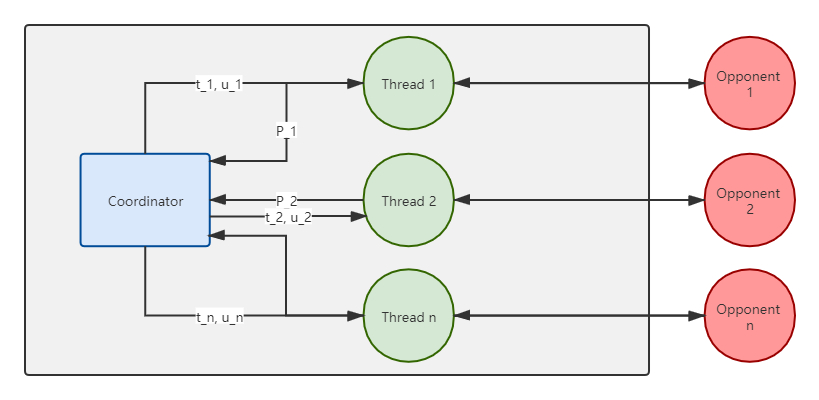
\includegraphics[width=0.8\textwidth]{./images/heuristic_concurrent_negotiation.png}
\caption{Architecture of the concurrent negotiation agent, best time: $t_i$ and utility value: $u_i$, probability distributions: $P$ \parencite{Williams12Concurrent}.}
\label{fig:heuristic-concurrent-negotiation}
\end{figure}

\textbf{Negotiation Threads:}The strategy of each negotiation thread is an extension of a recently published, principled, adaptive bilateral negotiation agent. This agent was designed to be used in a similarly complex environment, but only for negotiations against a single opponent.

\textbf{Coordinator:}The role of the coordinator is to calculate the best time, $t_i$ and utility value, $u_i$ at that time, for each thread. To do so, it uses the probability distributions received from the individual threads, which predict future utilities offered by the opponents.

%\subsection{Optimal Negotiation Strategies}
\subsection{Conclusion}
From the analysis of the heuristic negotiation strategy in a specific field, we can get some important parameters, such as time, offer by opponent, that need to be considered as the information used in the \gls{rl} algorithm.

\section{Reinforcement Learning used in Autonomous Negotiation}
\textbf{\gls{negosi}:} A novel algorithm named negotiation-based MARL
with sparse interactions (NegoSI) is presented by \texttt{Luowei Zhou}. In contrast to traditional sparse-interaction based MARL algorithms, NegoSI adopts the equilibrium concept and makes it possible for agents to select the non-strict Equilibrium Dominating Strategy Profile (non-strict EDSP) or Meta equilibrium for their joint actions \parencite{L2017NegoSI}.


\textbf{\gls{rlboa}:} From the paper \parencite{Bakker2019RLBOAAM} A Modular Reinforcement Learning Framework for Autonomous Negotiating Agents.

\textbf{\gls{anegma}:} Work by \parencite{bagga2020deep}. A novel DRL-inspired agent model called ANEGMA, which allows the buyer to develop an adaptive strategy to effectively use against its opponents (which use fixed-but-unknown strategies) during concurrent negotiations in an environment with incomplete information . 


\section{Challenges in Deep Reinforcement Learning}

\subsection{Sparse Reward}
Utility value as part of reward function
reward shaping
Curiosity Driven
Imitation Learning

\subsection{Non-stationary environment}
The strategy of single agent is changed during training
Multi-agent environment is non-statinal
Multi-agent deep reinforcement learning 

\subsection{Huge action space}
Action embedding, discrete action replaced by continious action space. 